%\documentclass[reprint,amsmath,amssymb,aps,twoside]{revtex4-2} % for editor use only

% For initial submission use these lines
\documentclass[amsmath,amssymb,aps,endfloats,linenumbers]{revtex4-2}


% DO NOT CHANGE THINGS BELOW HERE
\usepackage{graphicx}
\usepackage{amsmath,amssymb,amsfonts}
\usepackage{dcolumn}
\usepackage{bm}
\usepackage{siunitx}
\usepackage{booktabs}
%\usepackage{tikz,pgfplots}
\sisetup{separate-uncertainty=true, multi-part-units=single}
\usepackage[colorlinks,allcolors=blue]{hyperref}
\usepackage{cleveref}
\crefname{equation}{}{}
\crefname{figure}{Fig.}{Figs.}
\crefname{table}{Table}{Tables}
\usepackage{svg}
\svgpath{{./figures}}
\makeatletter
\def\blfootnote{\xdef\@thefnmark{}\@footnotetext}
\makeatother




% set PDF metadata
% AUTHORS EDIT THIS PART
\hypersetup{%
pdftitle={Verifying Tartaglia's Theory of Cannonball Motion}, % full title here
pdfauthor={Pranav Arunkumar, Lukas Fendrick, Sophia Maselli, Dylan Arello, Carter Krawiec}, % full author list here
}


\usepackage{fancyhdr}
\pagestyle{fancy}
\fancyhf{}
\fancyhead[RE,RO]{J S\&E \textbf{2}, xx--xx (2026)} % FOR EDITOR ONLY
\fancyhead[LO]{Arunkumar \emph{et al}} % if many authors
%\fancyhead[LO]{John and Dee} % if short enough to list all authors
\fancyhead[LE]{Verifying Tartaglia's Theory of Cannonball Motion} % full or short title depending on what fits
%\fancyhead[LE}{Several species of small furry animals gathered together in a cave and grooving with a pict} % might be too long
%\fancyhead[LE]{Several species grooving} % might be a short version of the title that fits
\fancyfoot[C]{\thepage}
\fancypagestyle{mytitlepage}{
\fancyhf{}
\fancyhead[C]{Journal of Science \& Engineering \textbf{2}, xx--xx (2026)} % FOR EDITOR ONLY
\fancyfoot[C]{\thepage}
\fancyfoot[L]{\scriptsize\copyright\ 2026 J S\&E \href{https://creativecommons.org/licenses/by-nc/4.0/}{CC-BY-NC 4.0}}
}


\begin{document}
%\setcounter{page}{67} % FOR EDITOR USE ONLY
%\linenumbers % FOR EDITOR USE ONLY

% AUTHORS EDIT THIS PART
\title{Verifying Tartaglia's Theory of Cannonball Motion}
\author{Pranav Arunkumar}
\altaffiliation{Manalapan High School} % use for non S&E authors
\author{Dylan Arello}
\author{Lukas Fendrick}
\author{Carter Krawiec}
\author{Sophia Maselli}
\email[Contact author: ]{428parunkumar@frhsd.com} % use FRHSD address
% For S&E authors
\affiliation{Science \& Engineering Magnet Program, \href{https://manalapan.frhsd.com/}{Manalapan High School}, Englishtown, NJ 07726 USA}
%\date{\today}
\received{13 May 2026} % FOR EDITOR USE ONLY
%\revised[revised~]{13 May 2026} % FOR EDITOR USE ONLY
\accepted[accepted~]{13 May 2026} % FOR EDITOR USE ONLY
\published[published~]{13 May 2026} % FOR EDITOR USE ONLY



% AUTHORS PUT YOUR MANUSCRIPT IN BELOW HERE
\begin{abstract}
  Nicolo Tartaglia theorized in his 1573 work \emph{Nova Sciencia} that projectiles travel furthest when shot at 45° and travel a linear trajectory before curving straight down. In this study, we tested his theories with modern physics models and determined that his theories do not hold true. We shot a 16mm stainless steel marble out of a PASCO ME-6825 launcher aimed at different angles and recorded the horizontal displacement for each. The data were then plotted in python and a regression was created based on modern mathematical models, as well as the residuals between for the regression. A Shapiro-Milk test of the residuals yielded a p-value of 0.06682, indicating our residuals were normally distrbuted and corroborated our modern model.

%\vspace{1em} % Add space before DOI
%\noindent DOI: \href{https://doi.org/10.64804/xxxxxx}{10.64808/xxxxxx}
\end{abstract}

% For revtex format this will not print on the article page but will be used in setting 
% the journal metadata so include keywords. Lowercase unless they are acronyms or proper nouns
% and pick keywords that will actually help people find your work properly. 
\keywords{kinematics, pop, time series}

\maketitle\thispagestyle{mytitlepage}
\blfootnote{\\\emph{Published by the Journal of Science \& Engineering under the terms of the \href{https://creativecommons.org/licenses/by-nc/4.0/}{Creative Commons Attribution-NonCommercial 4.0 International} license. Further distribution of this work must maintain attribution to the author(s) and the published article's title, journal citation, and DOI.}}

%The current column width is \the\columnwidth

\section{Introduction}
Nicolo Tartaglia was an Italian Renaissance mathematician, who was tasked with modeling the motion of cannonballs by the Doge of Venice in order to confer a military advantage. His predicted trajectory of cannonballs is as follows: first, the ball would move diagonally in a straight line, before curving in the arc of a circle and falling straight down as seen in \cref{fig:tart}.
\begin{figure}
\begin{center}
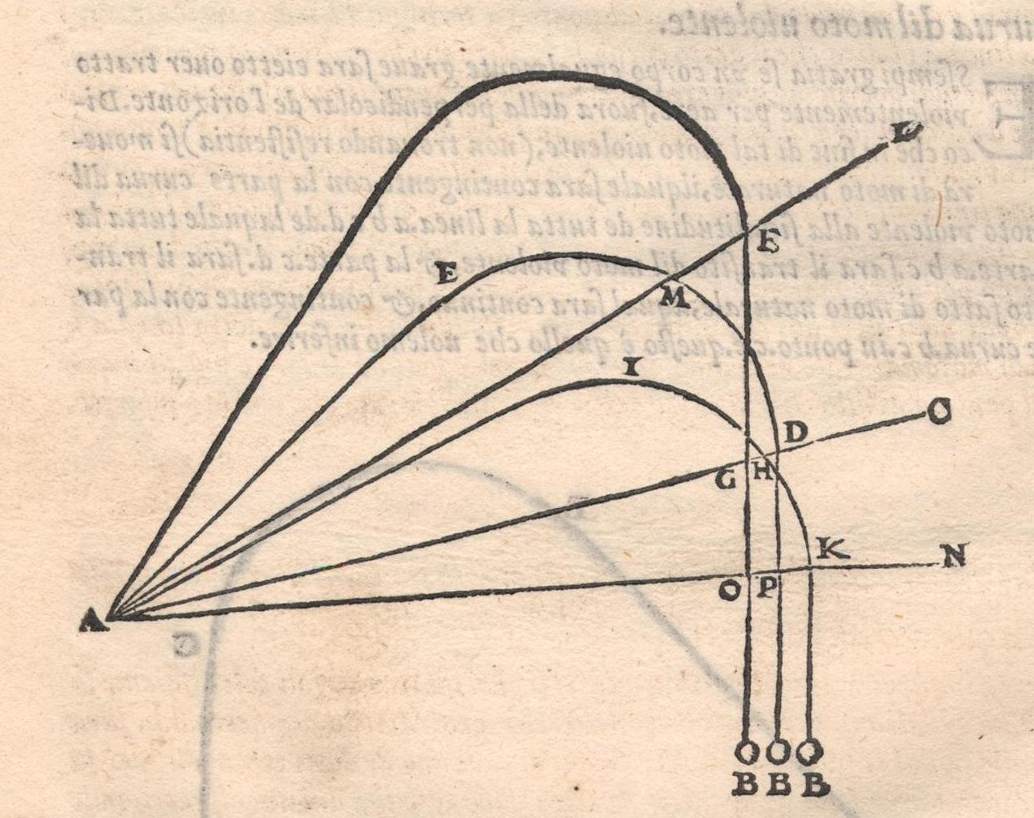
\includegraphics[width=0.99\textwidth]{figures/predicted_trajectory.jpg}
\end{center}
\caption{Tartaglia's prediction of cannonball flight in Nova Sciencia(1573)}
\label{fig:tart}
\end{figure}

He also predicted the horizontal ranges of cannonballs shot at various angles, concluding that they are symmetric at 45° and travel furthest at 45°. In this experiment, we aim to test his theories with more established mathematical models of projectile motion.

The position of a projectile--such as a cannon--can be calculated by splitting its position into horizontal and vertical positions, as seen in Equations \cref{eq:horizontal} and \cref{eq:vertical}, where $v_0$ represents the initial velocity of the projectile, $\theta$ represents the initial angle, and $x_0$ and $y_0$ represent the initial positions on their respective axis \cite{tipler}.
\begin{equation}
  x(t) = v_0\cos{\theta}t + x_0
\label{eq:horizontal} % Label
\end{equation}

\begin{equation}
  y(t) = v_0\sin{\theta}t-\frac{1}{2}gt^2 - y_0
\label{eq:vertical} % Label
\end{equation}

In order to calculate the horizontal range, we need to compute when $y(t)=0$ via quadratic formula, and substitute the resulting $t$ value into $x(t)$.

Doing so, we get our final equation for which we fitted the data to.

\begin{equation}
  displacement = v_0\cos{\theta}* \frac{-v_0\sin{\theta} - \sqrt{v^2\sin{\theta}^2 - 4(y_0)(-\frac{1}{2}g)}}{-g}
\label{eq:model}
\end{equation}



\section{Methods and materials}
We conducted this experiment using a PASCO ME-6825 Mini Launcher (PASCO Scientific, Roseville, California) alongside a 16mm stainless steel marble with an average mass of 16.7g across 7 marbles, weighed using a Digital Pro Pocket Scale (Smart Weigh, New York, NY). We used these materials to repeat our methods across three trials. We used a C-clamp to hold the launcher against the table to ensure it did not move much over the course of the experiment.
Setting this up, we used two meter sticks, one at the standard length of 100cm, and another snapped in half, measuring around 55cm. We lined these up next to each other to measure the distance the marble was shot out of our launcher.

We began each of our three trials by setting our mini launcher to be parallel to the ground, at an angle of 0°. We then inserted the marble into the launcher until it clicked once. We recorded each trial with the webcam of the Lenovo Ideapad 5i (Lenovo, Morrisville, North Carolina) at 30 FPS.
We would then shoot the marble, having a group member estimate the distance of the shot by recording the length at which the marble fell below the table. Then, using a protractor, we increased the angle by 7.5° and repeated the process again, eventually stopping the trial after 90°.

At a later point in time, we recorded a brief trajectory shot using an Arducam OV9281 1MP USB Camera (Arducam, Nanjing, China) set to 60FPS. We then extracted the frames via ffmpeg(v8.1.2) and superimposed the images via AstroImageJ\cite{Collins:2017:AstroImageJ}.

To perform statistical analysis, we plotted our data and created a regression model with the use of the NumPy, SciPy, and Matplotlib libraries\cite{numpy,scipy,matplotlib}.


All code and figures used in this paper can be found at \url{https://github.com/qazniak-bl/marble-lab}.

\section{Results}

The data in Table \cref{tab:projectile-distance} show our measurements across three trials at different angles and a calculated average horizontal range.

\begin{table}[htbp]
    \centering
    \caption{Marble Horizontal Range at Different Launch Angles}
    \label{tab:projectile-distance}
    \begin{tabular}{ccccc}
      % \centering
        \toprule
        Angle ($^\circ$) &
        Trial 1 (cm) &
        Trial 2 (cm) &
        Trial 3 (cm) &
        Average (cm) \\
        \midrule
        0.0  & 20  & 25  & 21  & 22.00 \\
        7.5  & 51  & 50  & 52  & 51.00 \\
        15.0 & 75  & 65  & 60  & 66.67 \\
        22.5 & 99  & 96  & 87  & 94.00 \\
        30.0 & 103 & 97  & 97  & 99.00 \\
        37.5 & 102 & 103 & 98  & 101.00 \\
        45.0 & 99  & 96  & 91  & 95.33 \\
        52.5 & 90  & 90  & 85  & 88.33 \\
        60.0 & 80  & 77  & 76  & 77.67 \\
        67.5 & 45  & 46  & 47  & 46.00 \\
        75.0 & 30  & 32  & 31  & 31.00 \\
        82.5 & 2   & 2   & 10  & 4.67 \\
        90.0 & 0   & 0   & 0   & 0.00 \\
        \bottomrule
    \end{tabular}
\end{table}

Using this data we used python to plot and create a regression function according to the model in Equation \cref{eq:model} via Scipy and Matplotlib\cite{scipy,matplotlib}.
Our regression is visible in \cref{fig:regression} and produced an estimated initial velocity ($v_0$) of 290.8049 cm/s and an estimated initial height of 8.7794 cm.
\begin{figure}
  \centering
    \includesvg[width=0.99\textwidth]{figures/Figure_1}
    \caption{Plot of horizontal range vs. degrees}
    \label{fig:regression}
\end{figure}

We used this same regression to generate a plot of the residuals, visible in \cref{fig:residual}.
\begin{figure}
  \centering
    \includesvg[width=0.99\textwidth]{figures/residuals_final}
    \caption{Plot of residuals}
    \label{fig:residual}
\end{figure}

To verify that the regression equation was a good fit for the data, we conducted a Shapiro-Wilk test on the residuals to assess their normality, with the null hypothesis being that if the regression is a good fit for the data, the residuals would be normally distributed. In doing so, we got a test statistic of 0.9473 and a p-value of 0.06682.

The super-imposed trajectory of the marble can be found in \cref{fig:trajectory}.
\begin{figure}
  \centering
  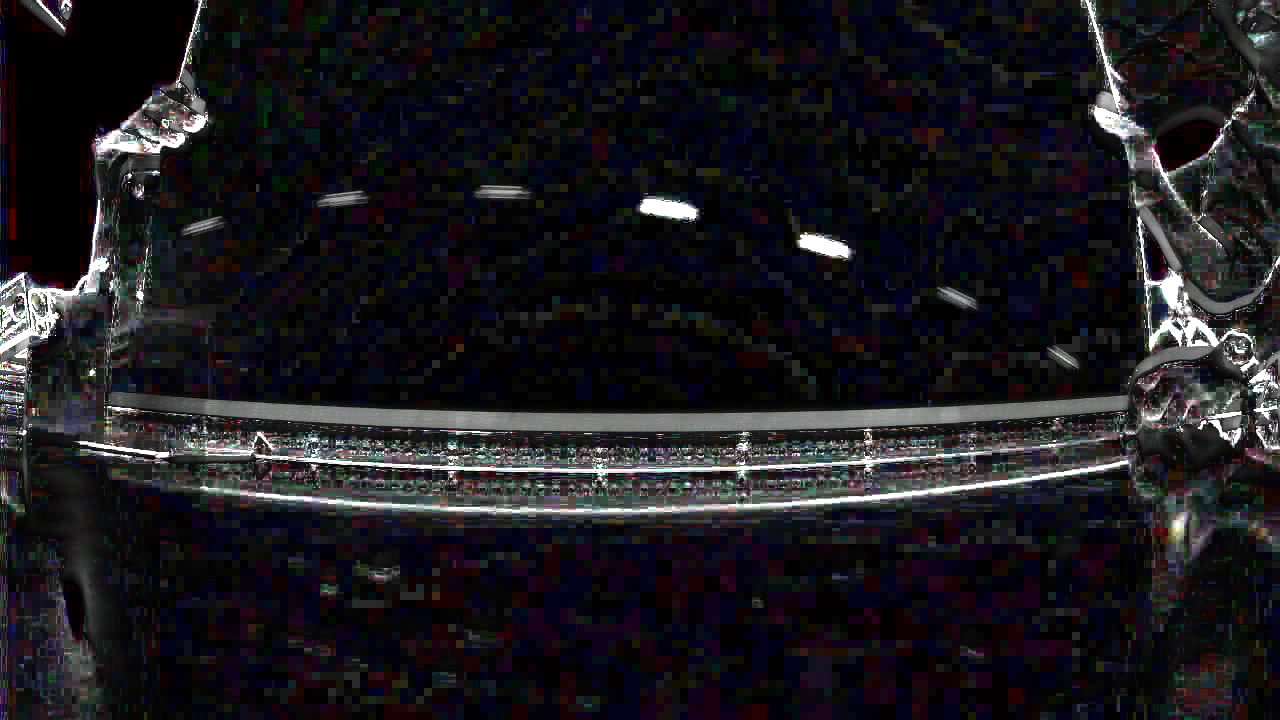
\includegraphics[width=1\textwidth]{figures/MAX_differenceStack.png}
  \caption{Trajectory of the marble}
  \label{fig:trajectory}
\end{figure}


    
\section{Discussion}
Our polynomial fit produces an $R^2$ value of 0.8971, which means that our model accounted for 89.71\% of the variation when we model horizontal range as a function of angle.
This indicates our model fit the data fairly well. The results of our Shapiro test also corroborate this: our p-value of 0.06682 is greater than our significance level of $\alpha=0.5$, so we have no reason to reject our null hypothesis that the residuals are normally distributed.

Furthermore, our trajectory found in \cref{fig:trajectory} is nothing like what Tartaglia predicted in \cref{fig:tart}. As such, we can discredit his second theory.

Tartaglia also predicted that horizontal range would be maximized at 45°, but our data in \cref{tab:projectile-distance} shows that horizontal range actually reached its maximum at 37.5°. Additionally, there is no obvious symmetry around the angle of maximum range, although this could be due to our lack of proper recording equipment.
As such, we conclude that Tartaglia's initial claim about the angle of maximum range was wrong, but we can not reliably deny his claim regarding the symmetry of the range.

We encountered a couple human errors as we did our tests and experiments. A major experience with these errors was a mistake we encountered while angling the cannon.
These measurements caused our own data tables to have a large margin of error as we progressed in our trials. Our cannon was supposed to start at 0°, incrementing by 7.5° for each shot until 90° is reached; however we ended up shortening the increment, and so, when we were intending to be at 90° when we were actually at around 80°.
To remedy this, we re-did our original trial. This took more time, and in hindsight we should have been more precise with our measurements. We also did not have the greatest tools to record the distance at which the marble fell below the table.

Additionally, the camera we used to map the trajectory of the marble (Arducam) had some lens distortion, resulting in a parabolic view of the shot. While we could have accounted for this, we had no need to, as this video was only used to map out the trajectory and not used to extract measurements.


\section{Acknowledgements}
SM tracked the motion of the marble and recorded the distance it traveled. LF recorded the videos and wrote part of the discussion. CK took turns launching the marble at various degrees in different trials. PA performed the data analysis and wrote up the results. DA ensured the marble did not stray too far from the site after each launch.



\bibliography{example}
%References
% [1] P.A. Tipler and G. Mosca. Physics for Scientists and Engineers, 5th ed. (W H Freeman and Company, New York, 2004).
%
%“De Caelo : Aristotle : Free Download, Borrow, and Streaming : Internet Archive.” Internet Archive, 2026, archive.org/details/decaelo00aris. Accessed 12 Jan. 2026.
%
%Galilei, G. Dialogues Concerning Two New Sciences (1638).
%
%Chazot, Christophe. FizziQ. 5.0.4, Trapèze. Digital, 2025, Apple App Store.


\end{document}
